% Source: graduate-coursework/Research/Intro_to_Agents/handouts/Part7_Parallelization.tex

\documentclass[border=4pt]{standalone}
\usepackage{amsmath,amssymb,amsfonts}
\usepackage[T1]{fontenc}
\usepackage{graphicx}
\usepackage{lmodern}
\usepackage{tikz}
\usepackage{xcolor}
\usetikzlibrary{shapes.geometric, arrows.meta, positioning, calc, fit, backgrounds, matrix, decorations.pathreplacing}

\definecolor{UofSCGarnet}{HTML}{73000a}
\definecolor{UofSCBlack}{HTML}{000000}
\definecolor{UofSCWhite}{HTML}{ffffff}
\definecolor{UofSCRose}{HTML}{CC2E40}
\definecolor{UofSCAtlantic}{HTML}{466A9F}
\definecolor{UofSCCongaree}{HTML}{1F414D}
\definecolor{UofSCHorseshoe}{HTML}{65780B}
\definecolor{UofSCGrass}{HTML}{CED318}
\definecolor{UofSCHoneycomb}{HTML}{A49137}
\definecolor{UofSC90Black}{HTML}{363636}
\definecolor{UofSC70Black}{HTML}{5C5C5C}
\definecolor{UofSC50Black}{HTML}{A2A2A2}
\definecolor{UofSCWarmGrey}{HTML}{676156}
\definecolor{UofSCSandstorm}{HTML}{FFF2E3}
\definecolor{UofSCDarkGarnet}{HTML}{570008}
\definecolor{UofSCAzalea}{HTML}{844247}

\tikzset{
    % Node styles - all with sharp corners
    agentbox/.style={
        rectangle,
        draw=UofSCGarnet,
        fill=UofSCSandstorm,
        thick,
        minimum width=2cm,
        minimum height=0.8cm,
        text centered,
        font=\footnotesize
    },
    processbox/.style={
        rectangle,
        draw=UofSCAtlantic,
        fill=UofSCWhite,
        thick,
        minimum width=2.5cm,
        minimum height=0.7cm,
        text centered,
        font=\footnotesize
    },
    syncbox/.style={
        rectangle,
        draw=UofSCCongaree,
        fill=UofSCCongaree!20,
        thick,
        minimum width=3cm,
        minimum height=0.5cm,
        text centered,
        font=\footnotesize\bfseries
    },
    resultbox/.style={
        rectangle,
        draw=UofSCHorseshoe,
        fill=UofSCGrass!30,
        thick,
        minimum width=2cm,
        minimum height=0.7cm,
        text centered,
        font=\footnotesize
    },
    % Arrow styles
    myarrow/.style={
        ->,
        >=Stealth,
        thick,
        UofSCBlack
    },
    dashedarrow/.style={
        ->,
        >=Stealth,
        thick,
        dashed,
        UofSC70Black
    },
    % Timeline styles
    timeline/.style={
        draw=UofSCBlack,
        thick,
        ->,
        >=Stealth
    },
    timeblock/.style={
        rectangle,
        draw=none,
        minimum height=0.5cm,
        text centered,
        font=\tiny
    }
}

\begin{document}
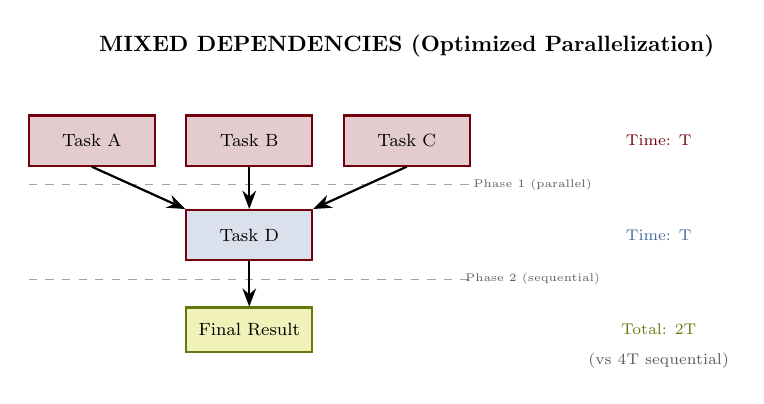
\begin{tikzpicture}[scale=0.8, transform shape]
            % Mixed dependency example
            \node[font=\bfseries] at (5,4.5) {MIXED DEPENDENCIES (Optimized Parallelization)};

            % Phase 1 - parallel
            \node[agentbox,fill=UofSCGarnet!20] (a) at (0,3) {Task A};
            \node[agentbox,fill=UofSCGarnet!20] (b) at (2.5,3) {Task B};
            \node[agentbox,fill=UofSCGarnet!20] (c) at (5,3) {Task C};

            % Phase 1 label
            \draw[dashed,UofSC50Black] (-1,2.3) -- (6,2.3);
            \node[font=\tiny,UofSC70Black] at (7,2.3) {Phase 1 (parallel)};

            % Phase 2 - depends on phase 1
            \node[agentbox,fill=UofSCAtlantic!20] (d) at (2.5,1.5) {Task D};

            % Phase 2 label
            \draw[dashed,UofSC50Black] (-1,0.8) -- (6,0.8);
            \node[font=\tiny,UofSC70Black] at (7,0.8) {Phase 2 (sequential)};

            % Result
            \node[resultbox] (result) at (2.5,0) {Final Result};

            % Arrows
            \draw[myarrow] (a.south) -- (d.north west);
            \draw[myarrow] (b.south) -- (d.north);
            \draw[myarrow] (c.south) -- (d.north east);
            \draw[myarrow] (d.south) -- (result.north);

            % Timing annotation
            \node[font=\scriptsize,UofSCGarnet] at (9,3) {Time: T};
            \node[font=\scriptsize,UofSCAtlantic] at (9,1.5) {Time: T};
            \node[font=\scriptsize,UofSCHorseshoe] at (9,0) {Total: 2T};
            \node[font=\scriptsize,UofSC70Black] at (9,-0.5) {(vs 4T sequential)};
        \end{tikzpicture}
\end{document}
